%%% Extra:
\textbf{Hasta 1.5pts extra.} Determina el código de tres direcciones
de la siguiente expresión,
\begin{center}
   $(a \ SUB \ b ) \ MOD \ ((MINUS \ c)  \ SUB \ d)$
\end{center}
usando las reglas semánticas siguientes. \\
Pueden omitir la explicación de la creación del árbol de sintaxis abstracta, 
pero hay que explicar los pasos del análisis semántico.

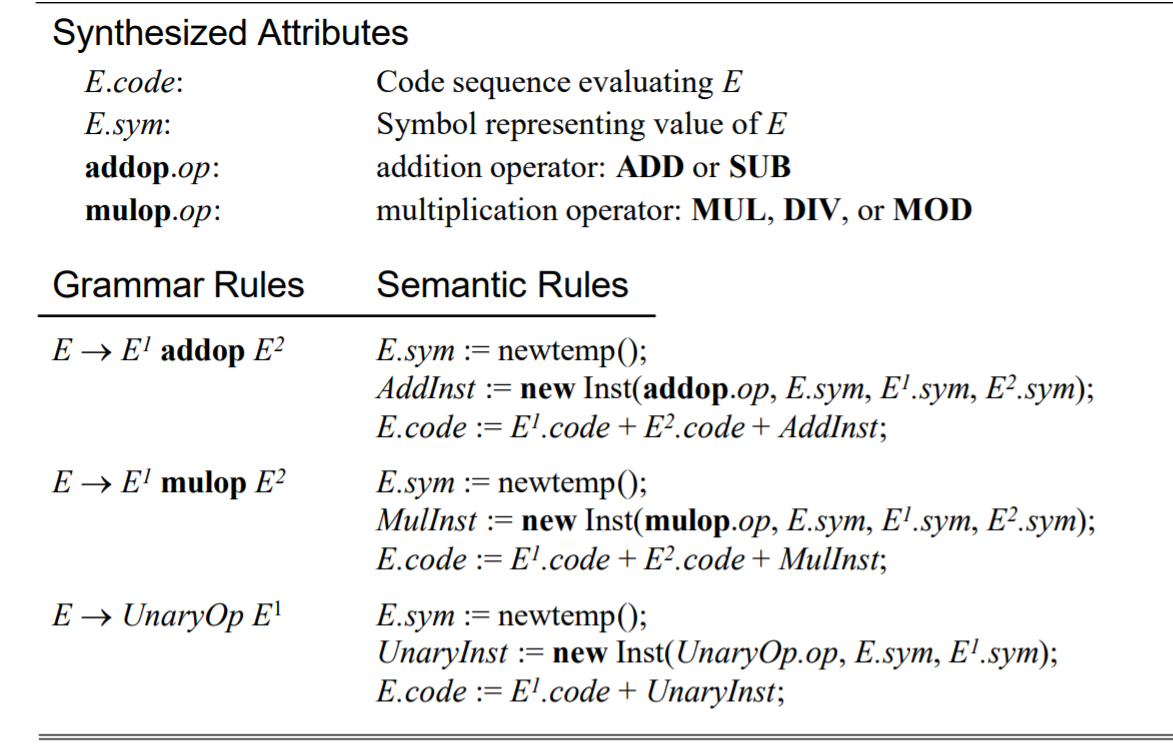
\includegraphics[width=0.7\linewidth]{./Fun_Sem_1.PNG}

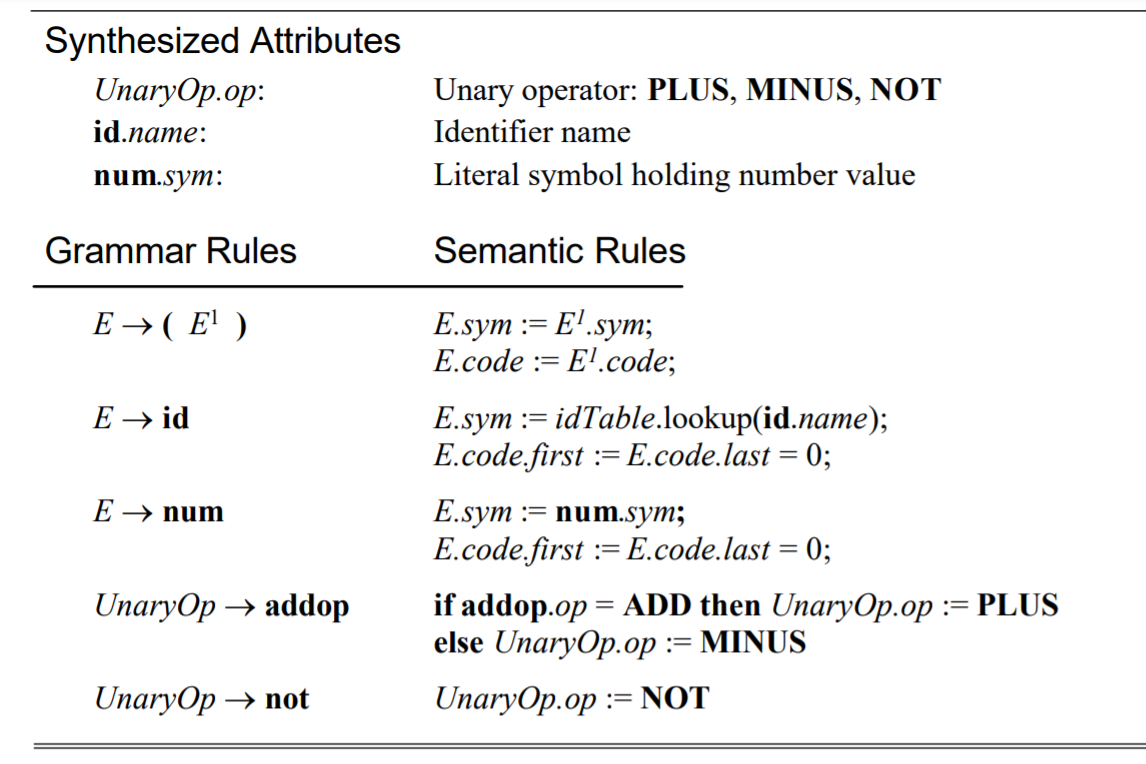
\includegraphics[width=0.7\linewidth]{./Funciones_Semanticas_2.PNG}
